\documentclass{beamer}
\usetheme{EMBL}
\definecolor{links}{HTML}{2A1B81}
\hypersetup{colorlinks,linkcolor=,urlcolor=links}
\usepackage{tikz}
\usepackage{lpc}
\usepackage{python}

\title[Jug]{Jug: Executing Parallel Tasks in Python}
\author{Luis Pedro Coelho}
\institute{EMLB}
\date{21 May 2013}

\def\iverson#1{%
\ensuremath{[}#1\ensuremath{]}%
}

\graphicspath{{figures/}{figures/generated/}{images/}}

\begin{document}
\frame{\titlepage}

\begin{frame}[fragile]
\frametitle{Jug: Coarse Parallel Tasks in Python}

\begin{itemize}
\item Parallel Python code
\item Memoization
\end{itemize}
\end{frame}

\begin{frame}[fragile]
\frametitle{Evaluating Segmentation Methods}

\begin{block}{Problem Statement}
\begin{enumerate}
\item You have images to segment
\item Many algorithms available
\item Which one is best?
\end{enumerate}
\end{block}

\pause

\begin{block}{Solution}
\begin{enumerate}
\item Manually segment a few images (reference)
\item Run algorithms on these images
\item Compare with reference
\end{enumerate}
\end{block}

\end{frame}

\begin{frame}[fragile]
\frametitle{Segmenting Images}

\centering
\includegraphics<1>[width=.7\textwidth]{image_stretched.jpeg}
\includegraphics<2>[width=.7\textwidth]{image_reference.jpeg}

\end{frame}


\begin{frame}[fragile]
\frametitle{Segmentation Live Demo}

If your software is really that good, you don't fear a live demo!

\end{frame}

\begin{frame}[fragile]
\frametitle{Methods}

\begin{python}
import mahotas as mh
def method1(image, sigma):
    image = mh.imread(image)[:,:,0]
    image  = mh.gaussian_filter(image, sigma)
    binimage = (image > image.mean())
    labeled, _ = mh.label(binimage)
    return labeled
\end{python}

\href{http://luispedro.org/software/mahotas}{mahotas} is my \alert{computer vision/image processing} package.

\end{frame}

\begin{frame}[fragile]
\frametitle{Segmentation Methods}


\begin{enumerate}
\item Threshold with Otsu
\item Threshold with mean
\end{enumerate}

\pause

\begin{itemize}
\item Neither of these methods is very good!
\item They are easy to explain \& demo
\item Read \href{http://www.ncbi.nlm.nih.gov/pmc/articles/PMC2901896/}{our paper} for what methods actually work.\\
(or just come talk to me).
\end{itemize}

\end{frame}

\begin{frame}[fragile]
\frametitle{Writing a jugfile}

\begin{block}{jugfile.py}
\begin{python}
from jug import TaskGenerator

@TaskGenerator
def method1(image, sigma):
    ...
\end{python}
\end{block}

\end{frame}


\begin{frame}[fragile]
\frametitle{Your code can be in multiple files}


\begin{block}{segmentation.py}
\begin{python}
import mahotas as mh

def method1(image, sigma):
    ...

\end{python}

\end{block}

\begin{block}{jugfile.py}
\begin{python}
from jug import TaskGenerator
from segmentation import method1

method1 = TaskGenerator(method1)

\end{python}
\end{block}
\end{frame}

\begin{frame}[fragile]
\frametitle{Comparing Automated \& Reference Segmentation}

\begin{python}
from glob import glob
inputs = glob('images/*.jpg')
results = []
for im in inputs:
    m1 = method1(im, 2)
    m2 = method2(im, 4)
    ref = im.replace('images','references').replace('jpg','png')
    v1 = compare(m1, ref)
    v2 = compare(m2, ref)
    results.append( (v1,v2) )
\end{python}

The above code looks like pure Python!
\end{frame}


\begin{frame}[fragile]
\frametitle{Demo Again}

Still working fine\ldots

\end{frame}


\begin{frame}[fragile]
\frametitle{Task hashing saves structure of computation}

\begin{block}{Let's look under the hood}
\begin{python}
@TaskGenerator
def double(x):
    return x*2

four = double(2)
eight = double(four)
\end{python}

\alert{converts to}

\begin{python}

def double(x):
    return x*2

four = Task(double, 2)
eight = Task(double, four)
\end{python}

\end{block}

\end{frame}

\begin{frame}[fragile]
\frametitle{Computation Structure}


\begin{center}
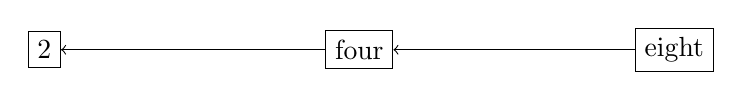
\begin{tikzpicture}
\node (two) at (0,0) [draw] {2};
\node (four) at (4,0) [draw] {four};
\node (eight) at (8,0) [draw] {eight};

\path[->]
    (four) edge (two);
\path[->]
    (eight) edge (four);
\end{tikzpicture}

\end{center}

\end{frame}

\begin{frame}[fragile]
\frametitle{Compute Hash}

\begin{python}
def hash-of(task):
    return crypto-hash( {
            task.function,
            task.args,
            task.kwargs })
\end{python}

\begin{itemize}
\item If \alert{task.args} are other tasks, recurse!
\item That's \alert{pseudo-code}
\item Real-life code \alert{slightly more complex}
\end{itemize}

\end{frame}

\begin{frame}[fragile]
\frametitle{The task hash encodes whole computation path}

\begin{python}
@TaskGenerator
def double(x):
    return x*2

four = double(2)
eight = double(four)
\end{python}

\begin{itemize}
\item \alert{four} encodes \verb+double(2)+
\item \alert{eight} encodes \verb+double(double(2))+
\end{itemize}

\end{frame}

\begin{frame}[fragile]
\frametitle{Running a Task}

\begin{python}
def maybe-run-task(task, backend):
    h = task.hash()
    if backend.can_load(h):
        # Nothing to do
        return
\end{python}
\pause
\begin{python}
    f = task.function
    args = []
    for a in task.args:
        if is-immediate-value(a):
            args.append(a)
        else:
            args.append(backend.load(a.hash()))
    # Same thing for kwargs
    return f(*args)

\end{python}

\begin{itemize}
\item Again, this is \alert{pseudo-code}
\end{itemize}

\end{frame}

\begin{frame}[fragile]
\frametitle{Two Backends Are Available}
\begin{block}{Filesystem}
\begin{itemize}
\item Default backend
\item Carefully designed to work on NFS
\item Anything pickle()able can be used as Task output/input.
\item Numpy arrays are special-cased (for speed and disk-space savings).
\end{itemize}
\end{block}

\begin{block}{Redis (NoSQL Database)}
\begin{itemize}
\item Redis is a file-backed store
\item Ideal for many small ``files''
\item All workers talk to same database
\end{itemize}
\end{block}

\end{frame}

\begin{frame}[fragile]
\frametitle{Jug Processes are Separate Processes!}
\begin{itemize}
\item \alert{No GIL (Global Interpreter Lock)} issues
\item Can run on \alert{separate machines}
\item Do not need to start at the same time
\end{itemize}
\end{frame}


\begin{frame}[fragile]
\frametitle{Invalidate All Downstream Results}
\begin{block}{Case Study}
\begin{enumerate}
\item You fix a bug in \alert{method1}.
\item Now, you need to recompute all \alert{method1} calls.
\item Also, \alert{print\_results}
\end{enumerate}
\end{block}
\end{frame}


\begin{frame}[fragile]
\frametitle{Jug Enhances Reproducibility}

\begin{block}{Typical \alert{Dark Side} of Computational Analysis}
\begin{itemize}
\item ``What was the parameter that generated this intermediate result?''
\item ``Deleted the intermediate results, reran; now everything is different.''
\item ``We cannot reproduce the table in our own paper.''
\end{itemize}
\end{block}

\begin{block}{Advantages of Jug}


\begin{itemize}
\item With jug, changing parameters \alert{will trigger recomputation of all
downstream results}.
\item \alert{jug invalidate} handles all dependencies
\item Unlike \alert{make}, you can use any Python function
\end{itemize}

\end{block}

\end{frame}
\begin{frame}[fragile]
\frametitle{How Much is Jug Used?}

\begin{itemize}
\item It started as stereotypical \alert{scratch an itch} software:\\
    I wrote it because I needed it
\item Not very widely used at the moment
\item Slowly picking up (by now 4.5 years old)
\item 43,000 PyPI downloads\\
    \alert{Was at 13,000 than a year ago}
\end{itemize}

\end{frame}

\begin{frame}[fragile]
\frametitle{Summary}
\begin{block}{Jug is Good For}
\begin{itemize}
\item Coarse tasks (at least 1 second, ideally a few more)
\item Data that fits on one disk
\item Fan-out/Reduce/Fan-out modes
\item Batch systems with shared network filesystems
\end{itemize}
\end{block}

\begin{block}{Jug is Not Appropriate For}
\begin{itemize}
\item Parallelization at micro level
\item Data that does not fit in one disk
\end{itemize}
\end{block}
\end{frame}

\begin{frame}[fragile]
\frametitle{Finding Out More About Jug\ldots}
\begin{itemize}
\item \url{http://metarabbit.wordpress.com}\\My blog, latest posts are about jug
\item \url{http://github.com/luispedro/jug}\\the code
\item \url{http://jug.rtfd.org}\\read the fine documentation
\item \url{http://groups.google.com/group/jug-users}\\google mailing list
\item \url{http://luispedro.org/software/jug}
\item luis@luispedro.org
\end{itemize}

\end{frame}

\end{document}

